\documentclass{report}
\usepackage[utf8]{inputenc}
\usepackage[a4paper, total={170mm,220mm}]{geometry}
\usepackage{titlesec}
\usepackage{multirow}
\usepackage{graphicx}
\titleformat{\chapter}[display]
  {\normalfont\bfseries\centering}{\LARGE Experiment\hspace{0.2cm} \thechapter }{0 pt}{\Huge}
  \titlespacing{\chapter}{0pt}{0pt}{8pt}  
\usepackage{fancyhdr}
\pagestyle{fancy}
\fancyhf{}
\fancyhead[RO,LE]{\thepage}
\renewcommand{\chaptermark}[1]{\markboth{#1}{#1}}
\fancyhead[CO,CE]{\leftmark}
\usepackage[framemethod=TikZ]{mdframed}
\usepackage{amsmath}
\usepackage{newtxtext,newtxmath}
\usepackage{float}
\newcommand{\toclineinsert}[3][25mm]{%
    \dotfill\ #2\makebox[#1][l]{#3\dotfill}%
}

\begin{document}



\tableofcontents


\chapter*{Critical solution Temperature}
\addcontentsline{toc}{chapter}{Critical solution Temperature \toclineinsert{}{21-11-2023}}
\begin{center}
    \LARGE
     \textbf{Date - 21-11-2023}
\end{center}

\section*{Aim}

To determine critical solution Temperature of phenol water system and variation of CST in presence of KCl

\section*{Principle}

The Temperature at which two partially miscible liquids becomes completely miscible is called critical solution temperature. Mixtures of phenol and different compositions of water is taken and their miscibility temperatures are plotted against their compositions.The maximum temperature point on the curve obtained is the critical temperature.\\
The critical solution temperature of the partially miscible liquids in fixed proportion increases linearly with the concentration of the impurity soluble only in one liquid.
\section*{Procedure}

5 ml of phenol is taken in a boiling tube. 2 ml of water is added to it from burette. It is stirred well and the temperature at which two liquids becomes completely miscible is noted. The mixture is then cooled by an air jacket and the temperature at which the turbidity appears is noted. The average of the two values is taken as the miscibility temperature. The experiment is repeated by adding 2 ml 

 \section*{Observation}

 \subsection*{Phenol-Water System}
\begin{table}[H] 
    \centering
\begin{tabular}{|l|l|l|l|l|l|}
\hline
Trial no: & Phenol & water & Disappear & Appear & Miscible temperature  \\ \hline
1         & 5 ml   & 2 ml  & 53.8      & 52     & 53.85 \\ \hline
2         & 5 ml   & 2 ml  & 54.4      & 54.5   & 54.45 \\ \hline
3         & 5 ml   & 4 ml  & 65        & 64     & 64.5  \\ \hline
4         & 5 ml   & 4 ml  & 66        & 65     & 65.5  \\ \hline
5         & 5 ml   & 6 ml  & 67        & 67.3   & 67.15 \\ \hline
6         & 5 ml   & 6 ml  & 67        & 68     & 67.5  \\ \hline
7         & 5 ml   & 8 ml  & 68        & 69     & 68.5  \\ \hline
8         & 5 ml   & 8 ml  & 69        & 69.7   & 69.35 \\ \hline
9         & 5 ml   & 10 ml & 69.6      & 69.5   & 69.55 \\ \hline
10        & 5 ml   & 10 ml & 69.1      & 70     & 69.6  \\ \hline
11        & 5 ml   & 12 ml & 70        & 70.5   & 70.25 \\ \hline
12        & 5 ml   & 12 ml & 70.5      & 71.2   & 70.85 \\ \hline
13        & 5 ml   & 14 ml & 71        & 70     & 70.5  \\ \hline
14        & 5 ml   & 14 ml & 69.1      & 69.8   & 69.45 \\ \hline
15        & 5 ml   & 16 ml & 69        & 68     & 68.5  \\ \hline
16        & 5 ml   & 16 ml & 69        & 67.8   & 68.4  \\ \hline
17        & 5 ml   & 18 ml & 68        & 67     & 67.5  \\ \hline
18        & 5 ml   & 18 ml & 67        & 67.5   & 67.25 \\ \hline
19        & 5 ml   & 20 ml & 66        & 65     & 65.5  \\ \hline
20        & 5 ml   & 20 ml & 65        & 66     & 65.5  \\ \hline

\end{tabular}

\end{table}
\begin{figure}[H]
    \centering
    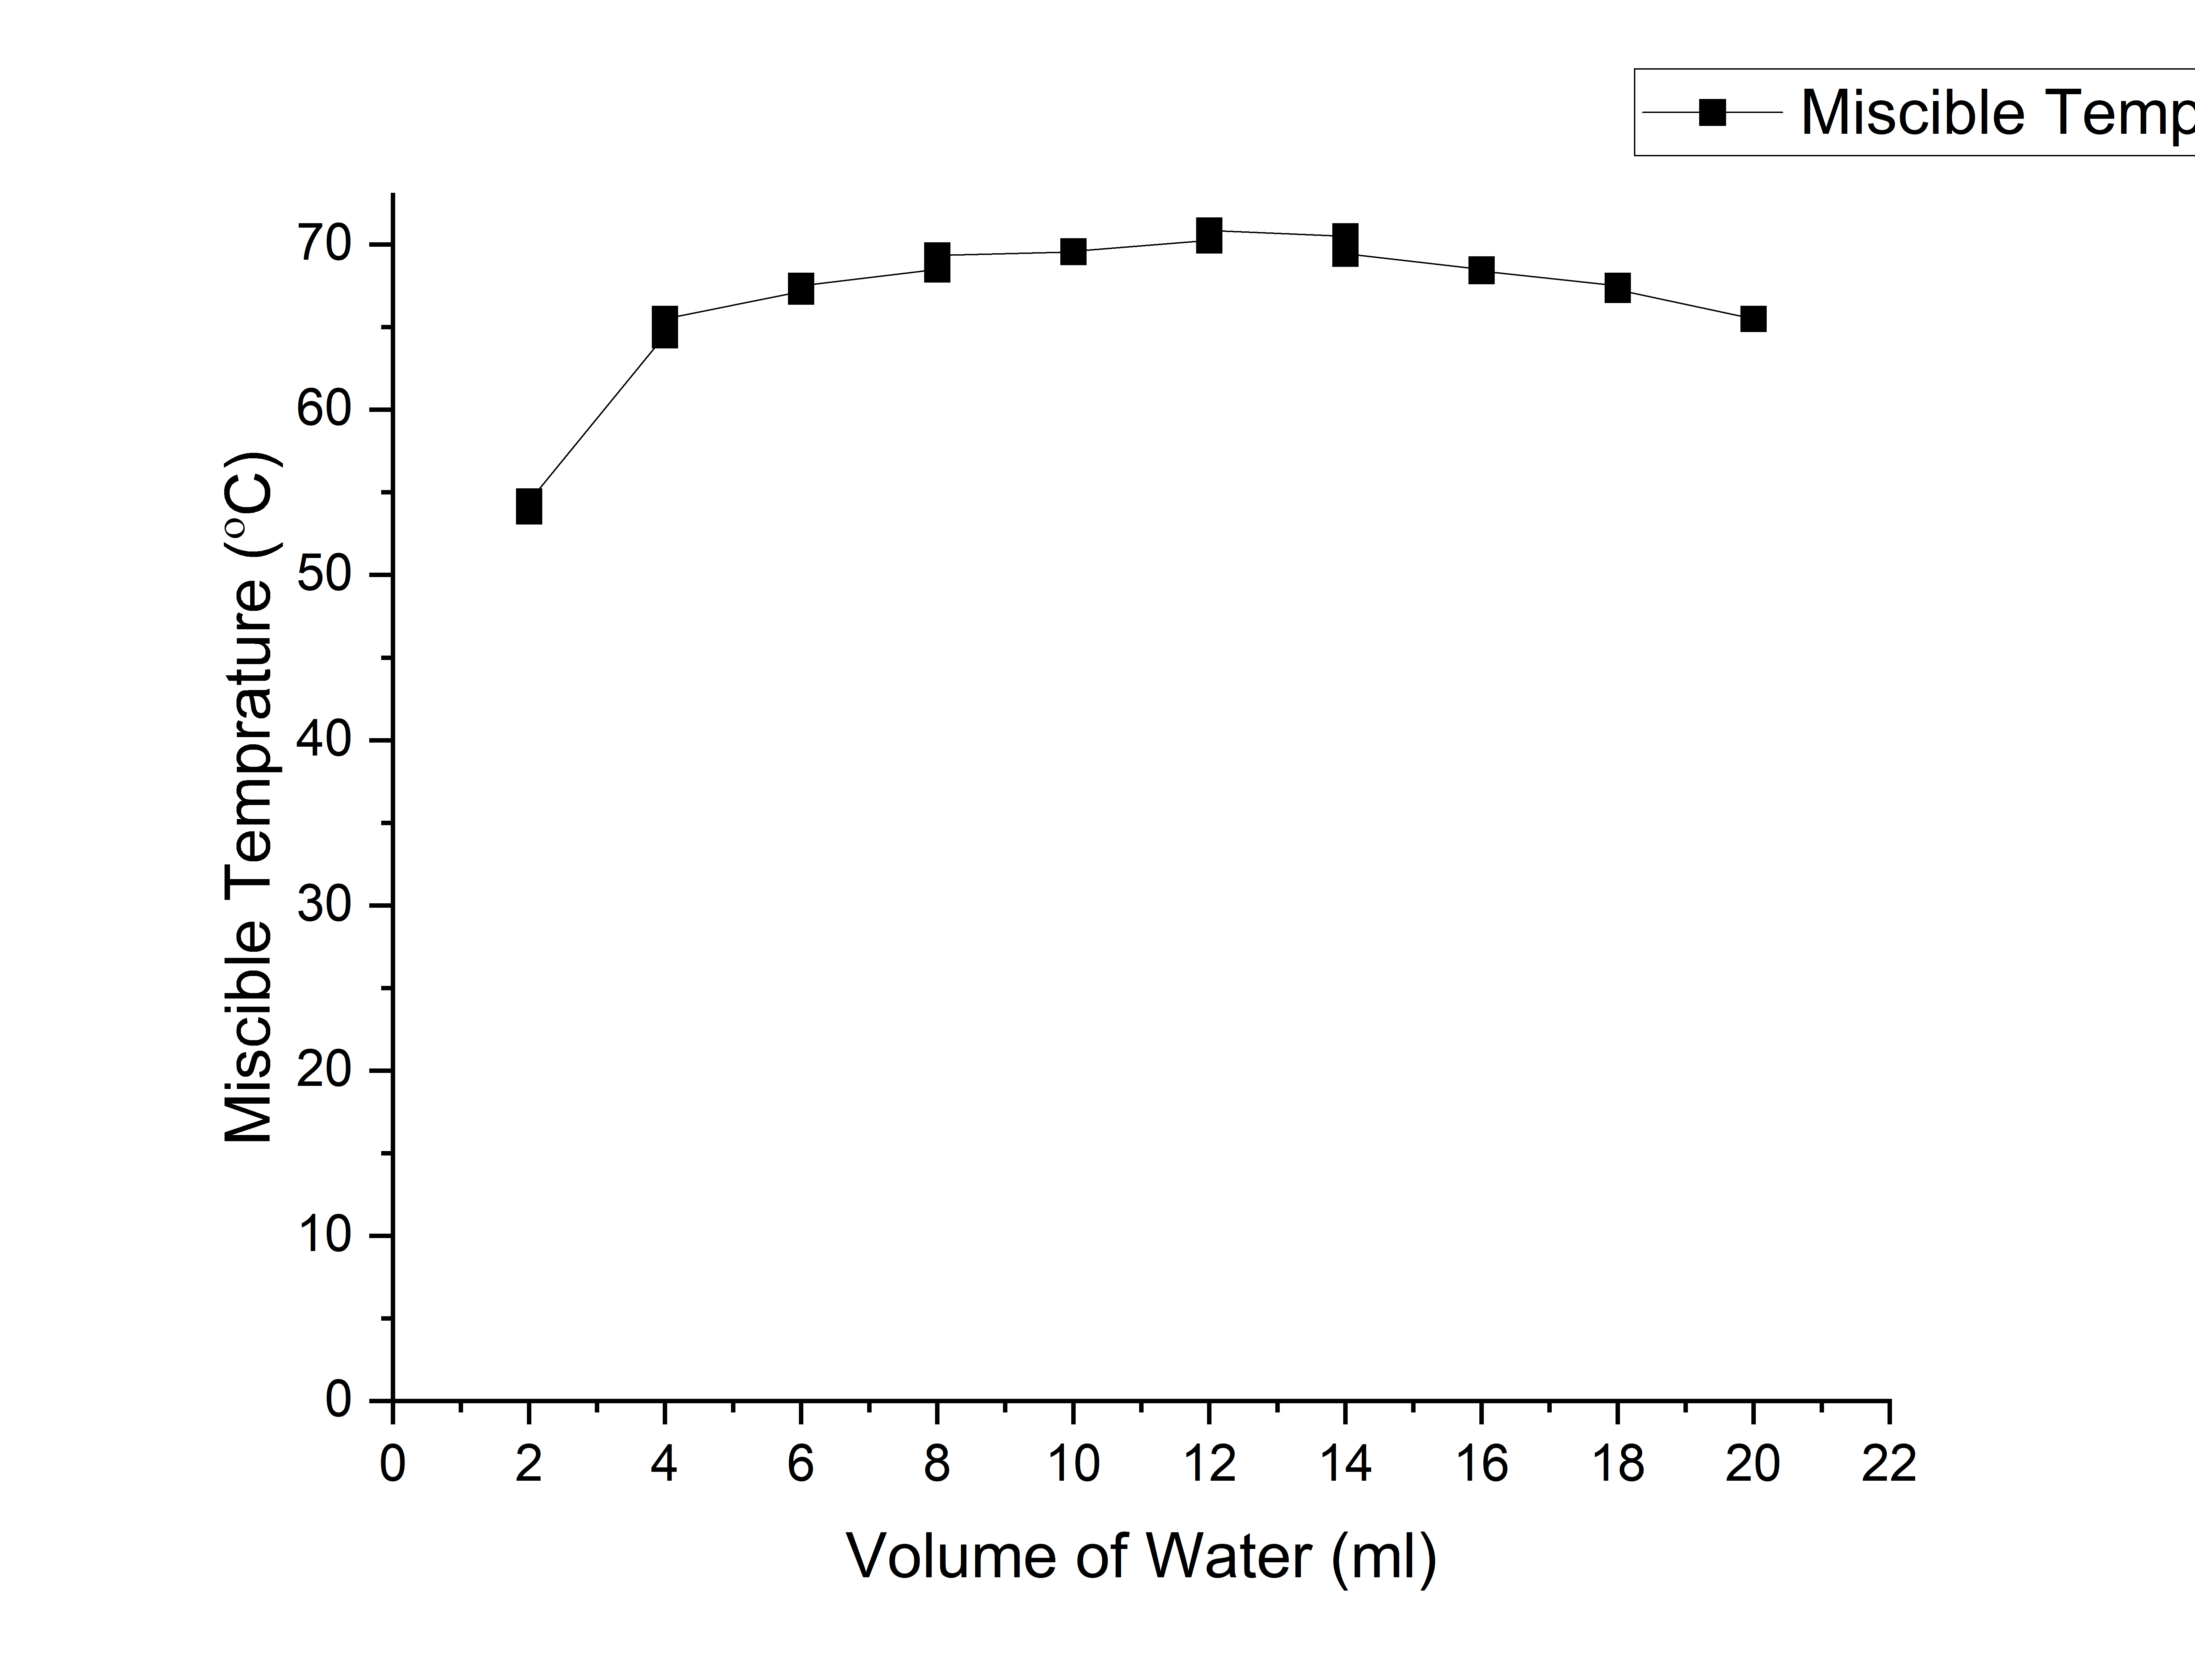
\includegraphics[width = 15cm]{cst-pheonl-water.png}
    \caption{Miscibility temparture vs Volume of Phenol in water}
\end{figure}

\subsection*{Effect of KCl on Phenol Water System}
\begin{table}[H]
\begin{tabular}{|l|l|l|l|l|l|}
\hline
Trial no: & KCl   & phenol & Disappear & Appear & Miscible temperature  \\ \hline
1         & 5 ml  & 5 ml   & 76.5      & 76     & 76.25 \\ \hline
2         & 5 ml  & 5 ml   & 76        & 76     & 76    \\ \hline
3         & 10 ml & 5 ml   & 75        & 75     & 75    \\ \hline
4         & 10 ml & 5 ml   & 75        & 74     & 74.5  \\ \hline
5         & 15 ml & 5 ml   & 75        & 73     & 74    \\ \hline
6         & 15 ml & 5 ml   & 74.5      & 73     & 73.75 \\ \hline
7         & 20 ml & 5 ml   & 71.5      & 73     & 72.25 \\ \hline
8         & 20 ml & 5 ml   & 69        & 69.5   & 66.75 \\ \hline
\end{tabular}
\end{table}

\begin{figure}[H]
    \centering
    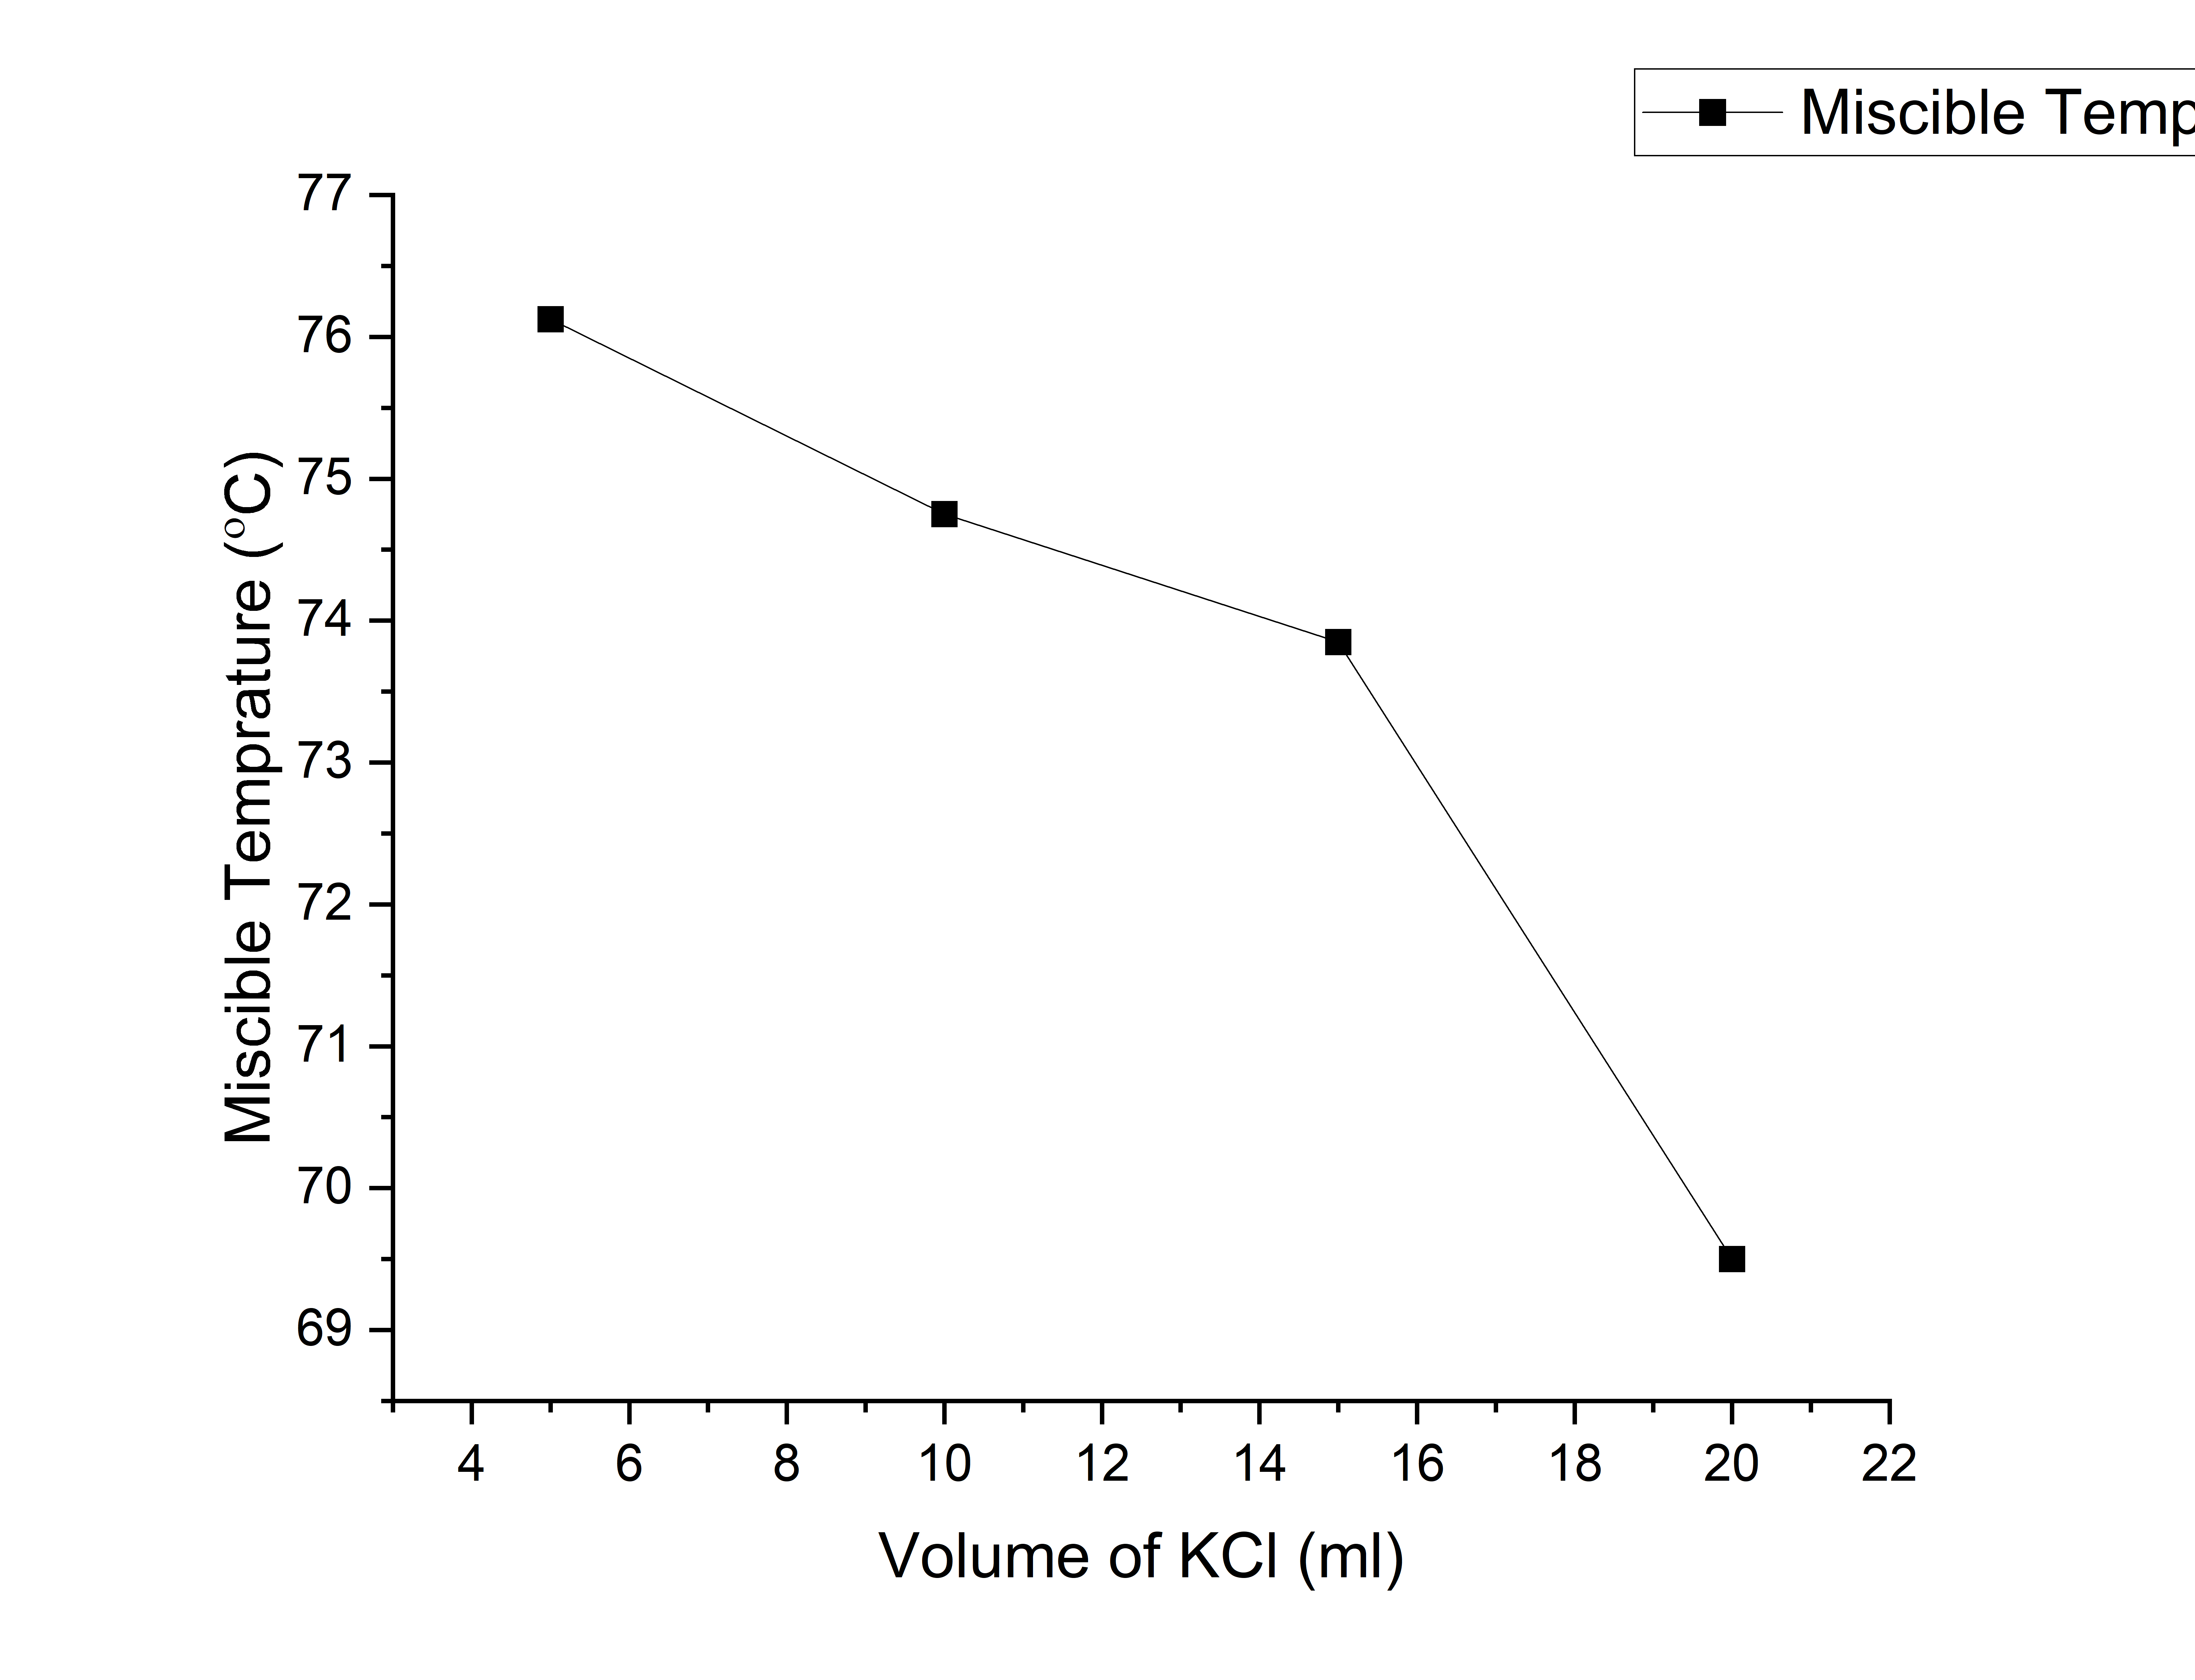
\includegraphics[width = 15cm]{cst-kcl.png}
    \caption{variation of CST pf Phenol-Water system with change in conc. of KCl}
\end{figure}


\section*{Result}
\begin{tabular}{l}
    The maximum of the graph gives CST of the phenol water system \\ 
    Critical solution temperature of phenol water system in degree celsius $= 76.25 ^\circ C$ \\
\end{tabular}


\chapter*{Composition From Viscosity Measurement}
\addcontentsline{toc}{chapter}{Composition From Viscosity Measurement \toclineinsert{}{5-12-2023}}

\begin{center}
    \LARGE
     \textbf{Date - 5-12-2023}
\end{center}

\section*{Aim}

Determine viscometrically the percentage composition of given sucrose solution.

\section*{Principle}

The viscosity of the solution increases with linearly with the concentration. By measuring the time of flow of the solution of different concentrations through a capilliary tube, a graph is drawn between time of flow and the percentage composition.From the graph, the concentration of the given solution can be found by measuring its time of flow.

\section*{Procedure}

Prepare sucrose solutions of different concentrations $1\%, 2\%, 3\%, 4\% $etc.  Using the the 15 percentage of stocks solution of sucrose the viscometer is cleared. It is dried and rinsed with the sugar solution. Pippetted volume (10ml) of the solution into the limb of the viscometer using a rubber tube. Suck the solution through the capilliary tube above the mark and release. When the solution just passes over the ,mark. Start stop watch and stop it when the solution just cross the mark below the bulb the time of flow is found out two or three times and the average time is found out clean the viscometer each time and dry or rinse when fresh solution is used. Repeat the experiment with sugar solution of known concentrations. A graph is drawn between the time of flow and percentage of composite. From the graph the percentage of composition of unknown solution is found out. 

\section*{Observation}

\begin{table}[H]
\begin{center}
\begin{tabular}{|c|c|c|}
\hline
No. & Composition $\%$ & Time of Flow (s)  \\ \hline
1   & 0                & 99                \\ \hline
2   & 1                & 95                \\ \hline
3   & 2                & 98                \\ \hline
4   & 3                & 99               \\ \hline
5   & 4                & 101               \\ \hline
6   & 5                & 103               \\ \hline
7   & 4                & 108               \\ \hline
\end{tabular}
\end{center}
\end{table}



\begin{figure}[H]
    \centering
    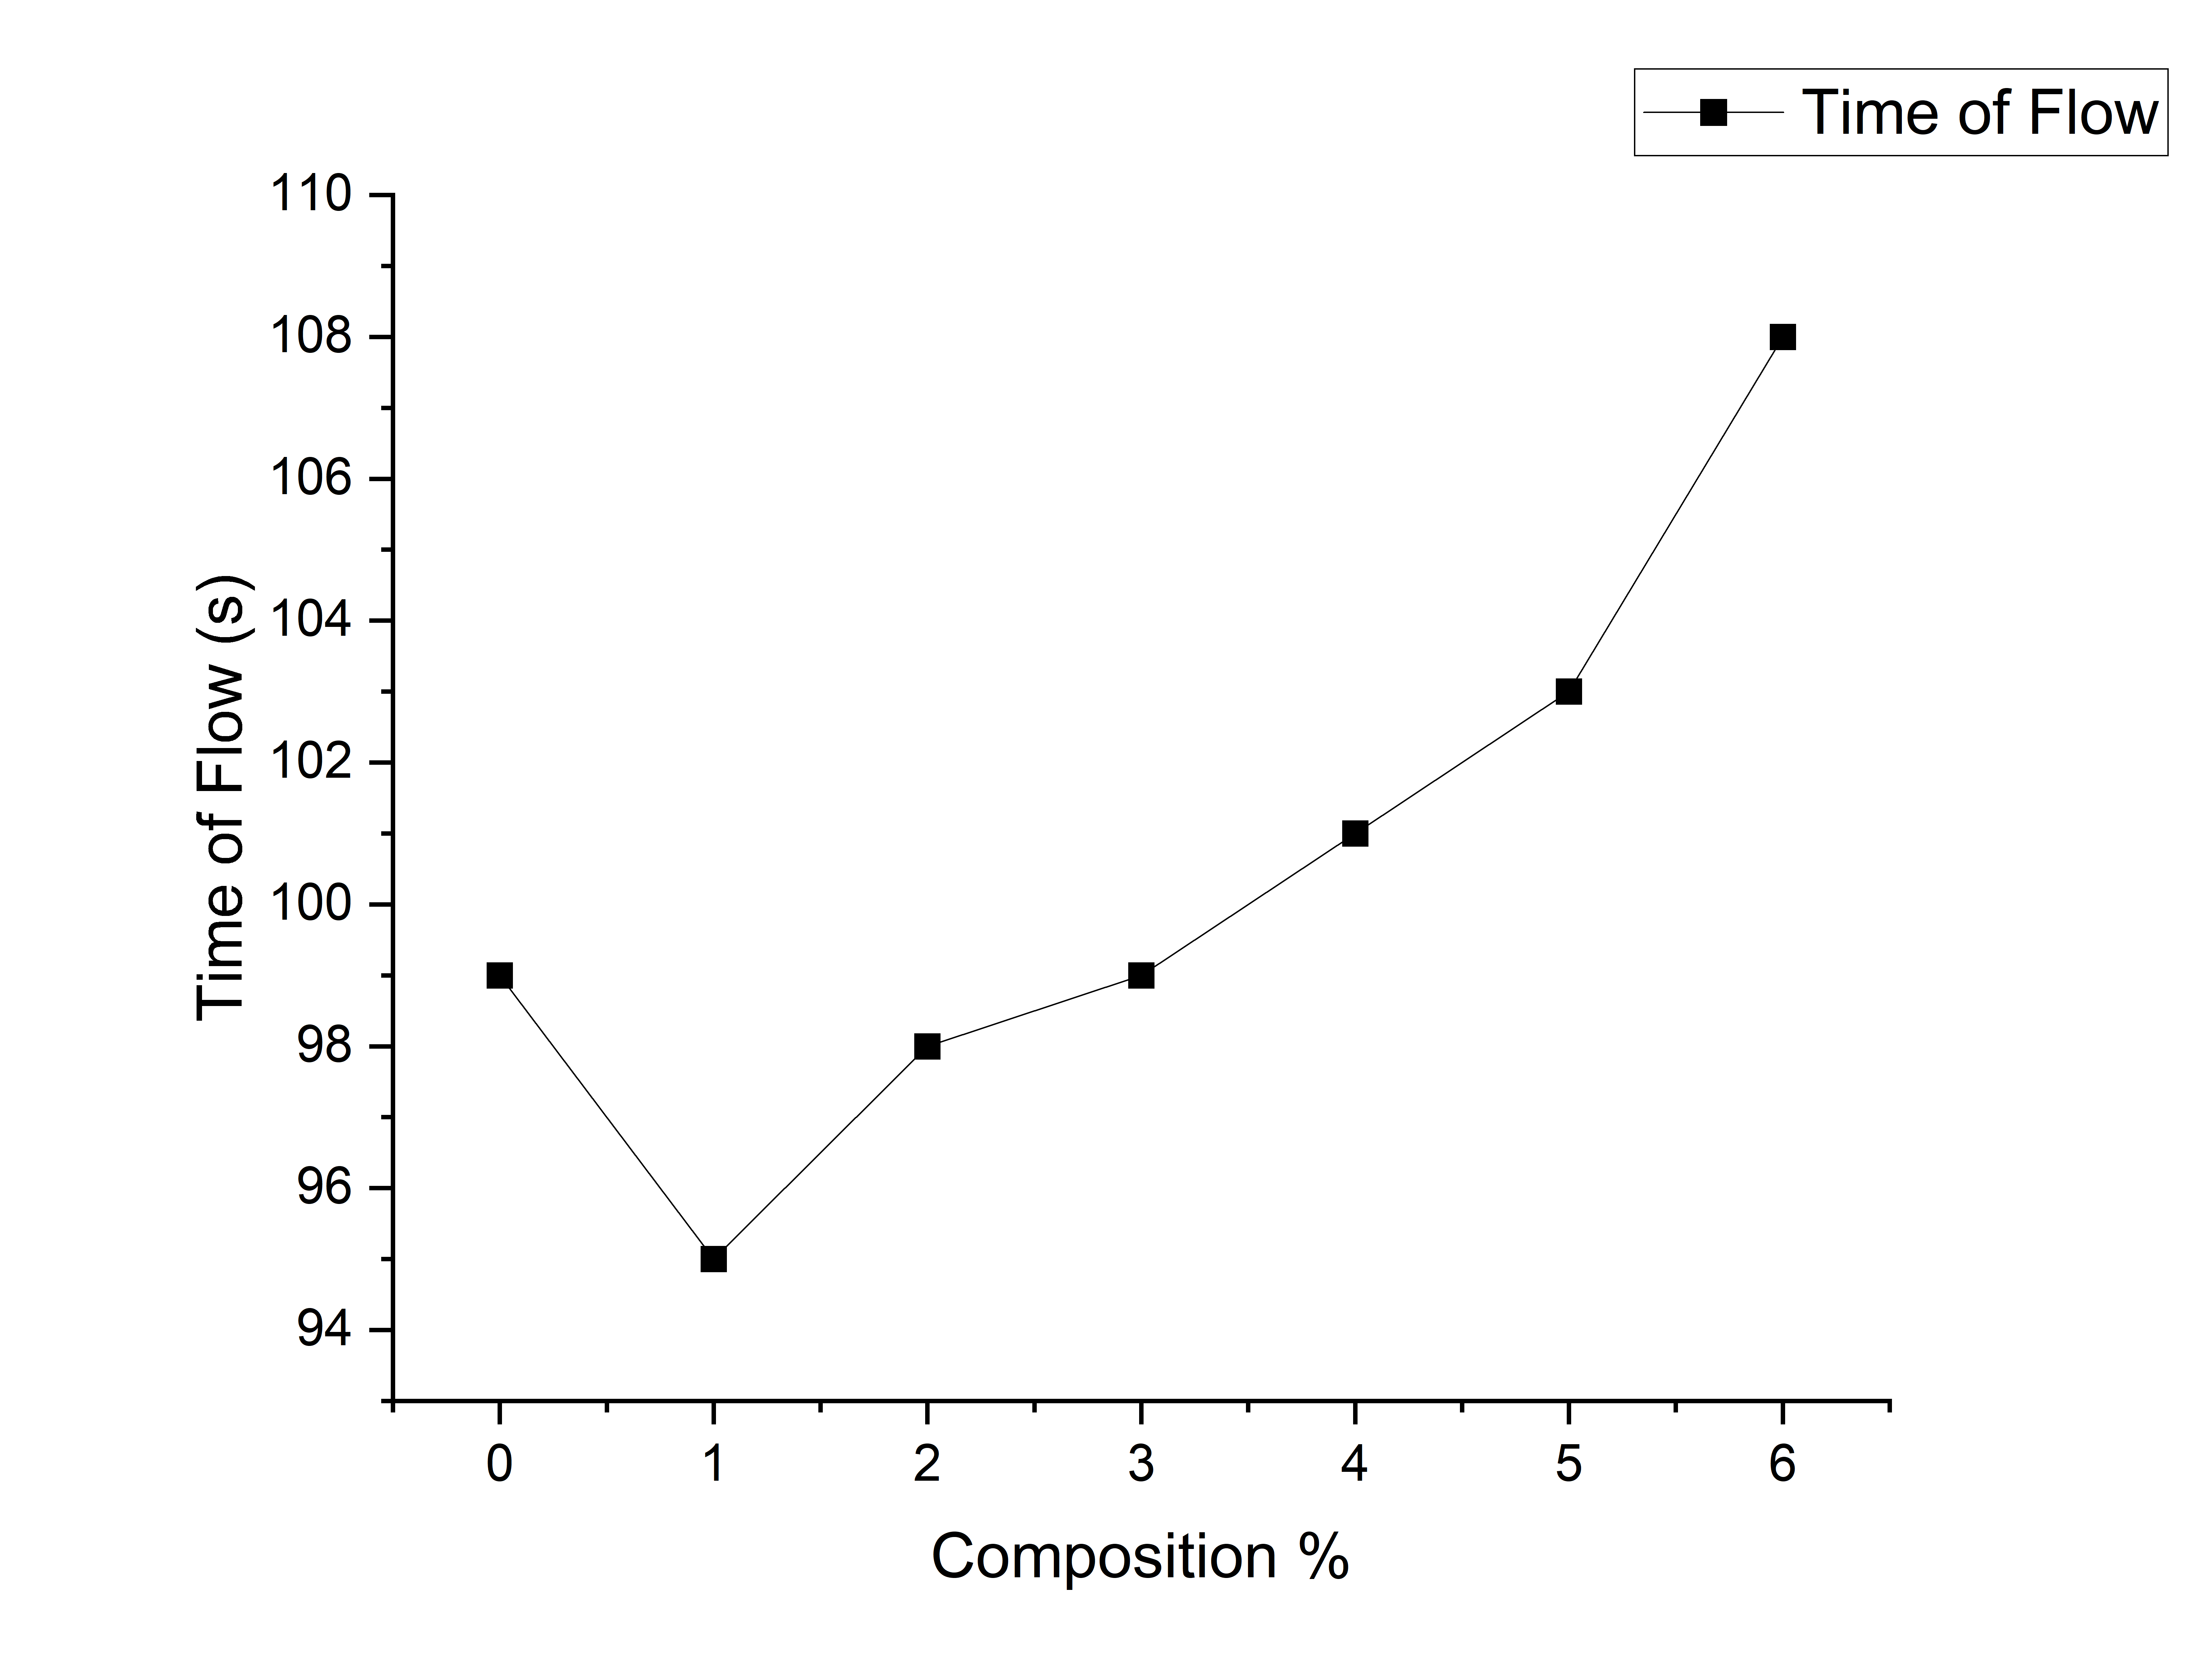
\includegraphics[width = 15cm]{viscocity.png}
    \caption{Composition percentage vs Time of Flow in seconds}
\end{figure}

\section*{Result}

The percentage composition of given solution is 4
\pagebreak


\chapter*{Caliberation of pH meter and Measurement of pH of solution}
\addcontentsline{toc}{chapter}{Caliberation of pH meter and Measurement of pH of solution\toclineinsert{}{5-12-2023}}

\begin{center}
    \LARGE
     \textbf{Date - 5-12-2023}
\end{center}

\section*{Aim}
To perform pH metric titration of a strong acid Hydrochloric acid with a strong alkali sodium hydroxide.


\section*{Principle}

The pH of a solution can be measured accurately with the help of a pH meter.Measurement of pH is employed to monitor the cause of acid-base titration. It affords a direct method of obtaining a titration curve. The titration curve is a graph of measured pH values versus the volutne (ml) of titrant added. The pH values of the solution at different stage of acid-base neutralization are determined and plotted against the volume of alkali added on adding a base to an acid, the pH rises slowly in the initial stages as the concentration of H+ ion decreases gradually due to the consumption of some amount of HCl by NaOH resulting in the formation of NaCl (whose amount will be the same as that of NaOH added).

$$HCl(aq)+NaOH(aq) NaCl(s)+H_2O(l) $$

\section*{Procedure}
A 0.1(M) HCl solution and unknown concentration of NaOH solution are given. With pH 4, 7, and 10 solutions, calibrate the pH metre. When cleaning the electrode,use purified water and tissue or filter paper. Place the electrode in a 25ml solution of NaOH in a 50ml beaker. Make a note of the pH range. Rinse the burette twice: once with HCl solution and once with distilled water. After that, pour HCl solution into the burette. The pH value of the NaOH solution is indicated by the reading on the pH meter's scale. Using a glass rod to vigorously stir the mixture, add drops of HCl solution from the burette (1ml at a time), then record the resulting pH values.
Because the acid is neutralised and there will be a dramatic increase in pH values near the end point, the volume of HCl administered should be as tiny as possible.

Even a small further addition of 1ml of HCl will raise the pH level to around 9-10.
After each pH measurement, reset the selection to its initial position, and maintain it there whenever it's not in use.

Plot the graph of pH of solution v/s volume of HCl in ml.

\section*{Observation}
\begin{table}[H]
\begin{tabular}{|l|l|l|}
\hline
\textbf{Sl.No.} & \textbf{Composition} & \textbf{pH of solution} \\ \hline
1               & HCl + 1 ml NaOH        &     12.02                    \\ \hline
2               & HCl + 2 ml NaOH        &     12.12                   \\ \hline
\end{tabular}
\end{table}

\begin{figure}[H]
    \centering
    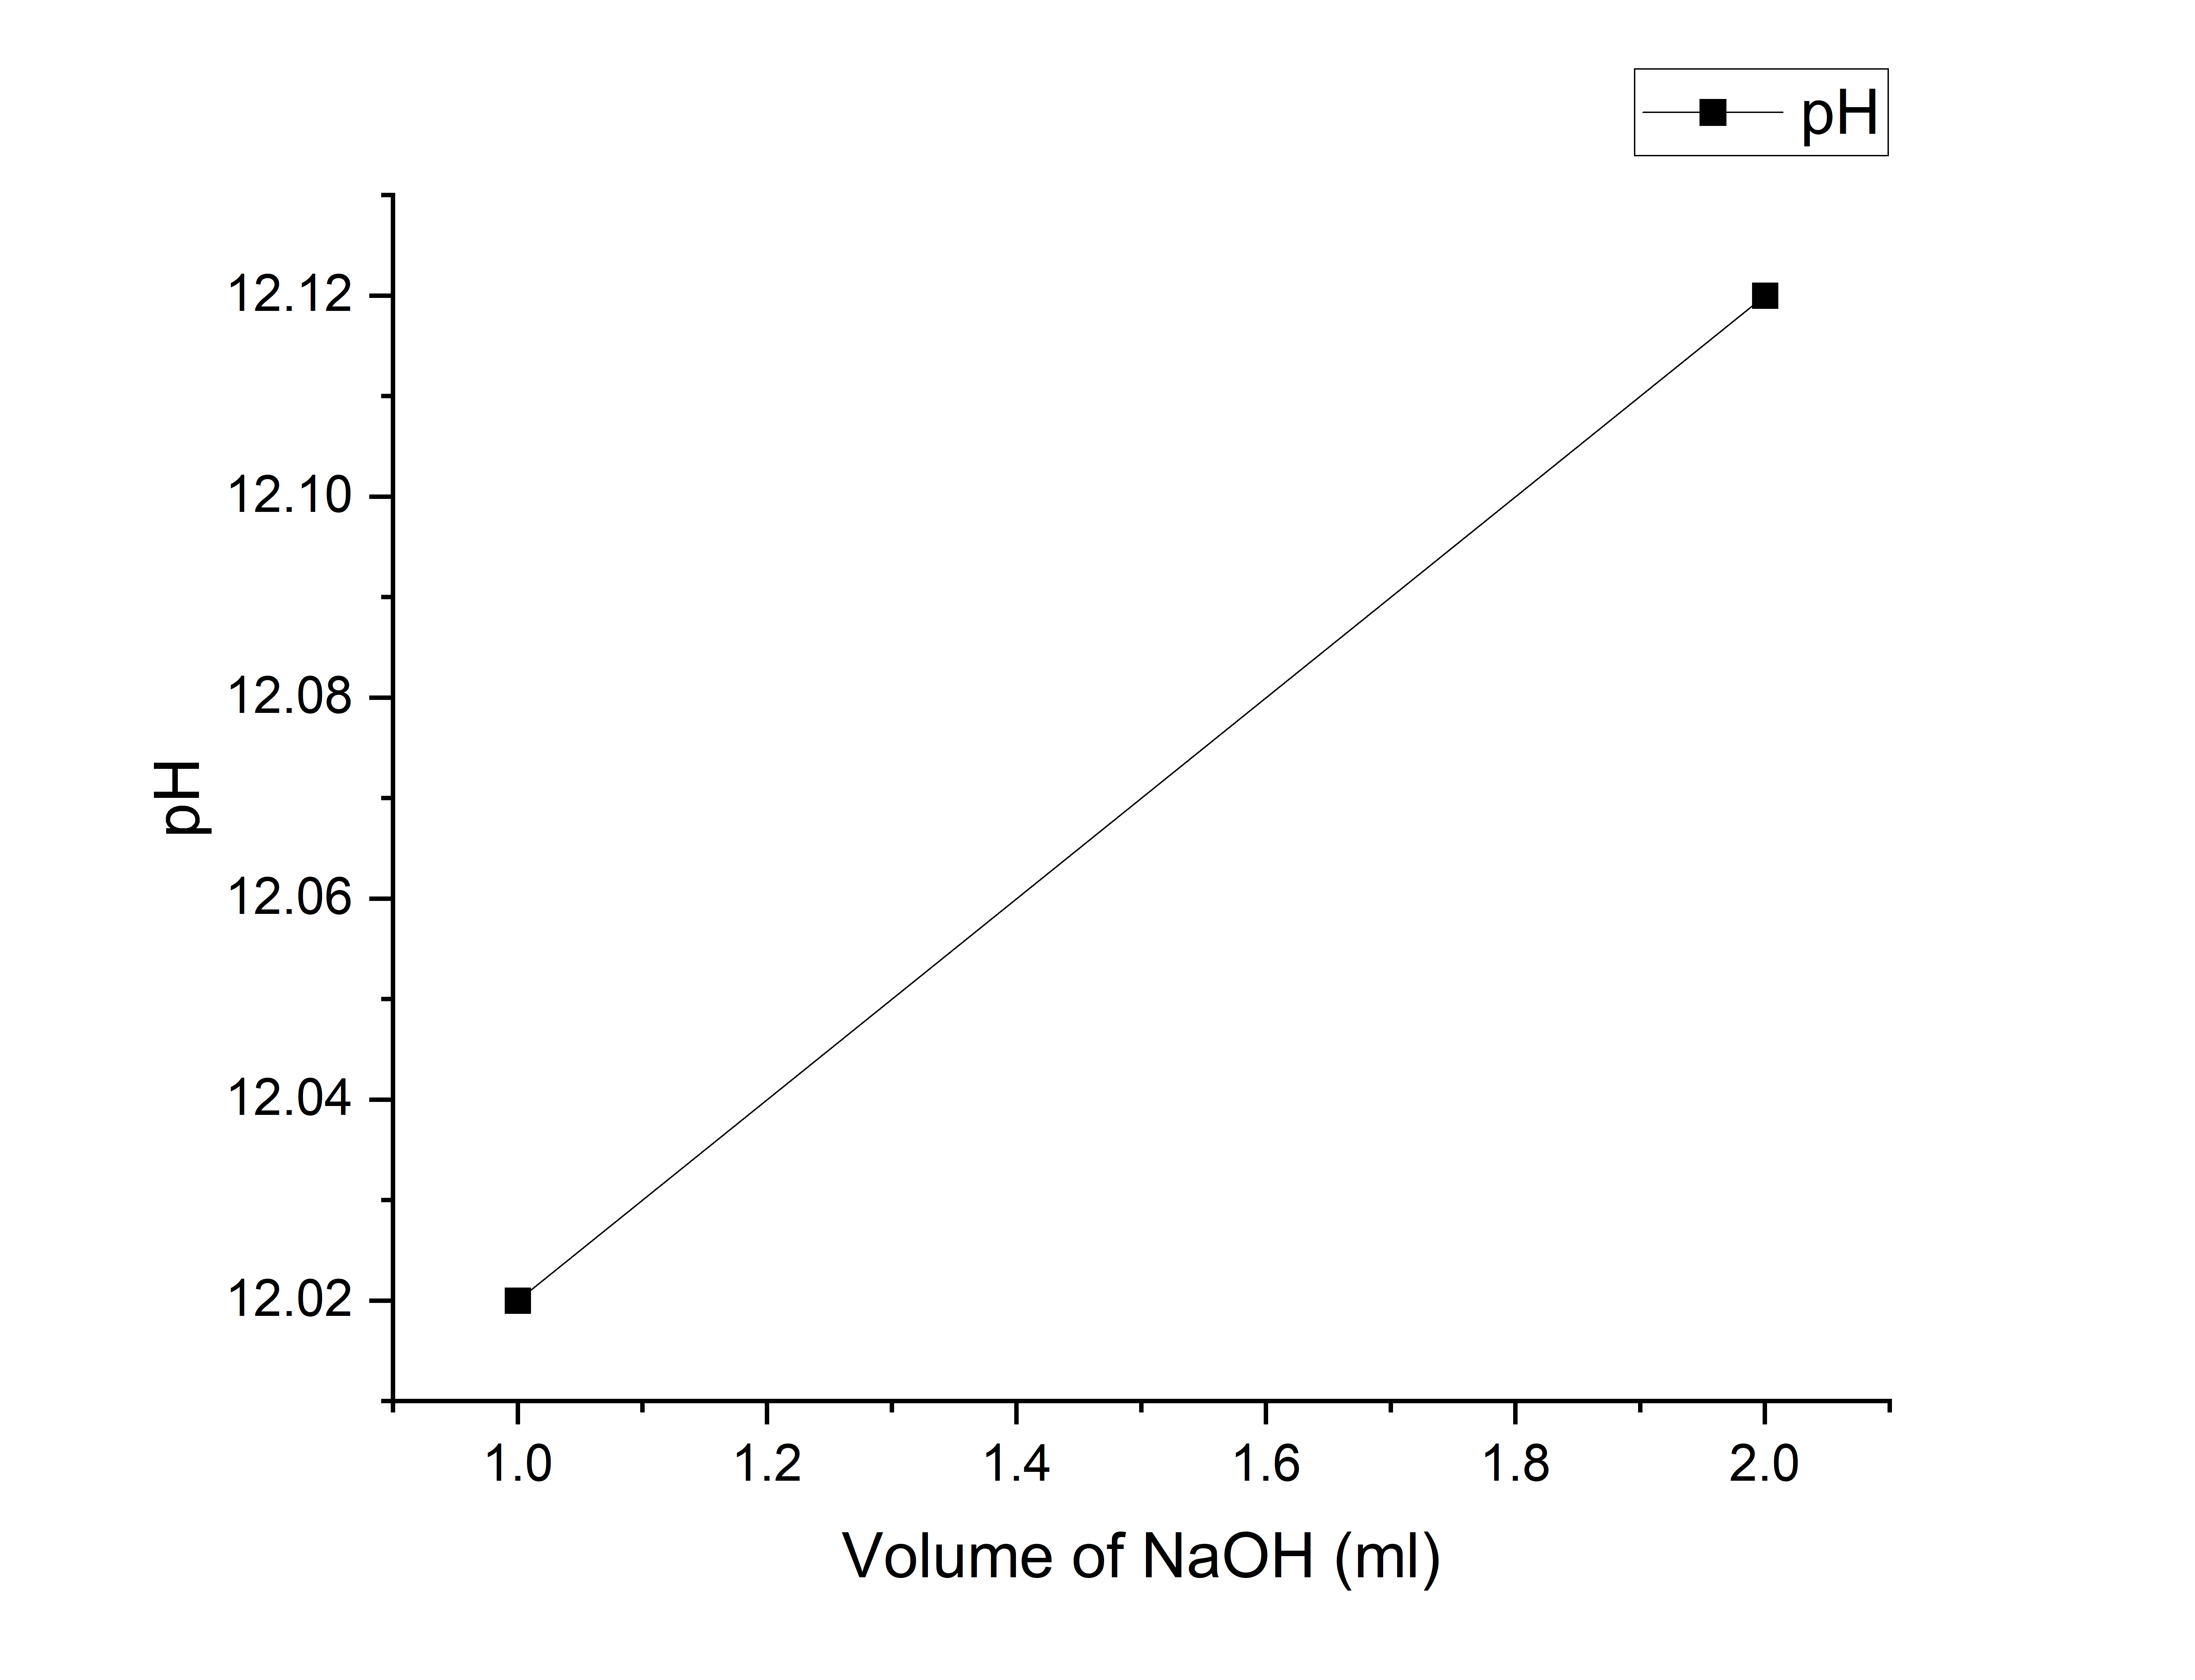
\includegraphics[width = 15 cm]{pH.png}
    \caption{Variation of pH with NaOH added}
\end{figure}

\section*{Result}
The graph of pH of solution v/s volume of HCl is plotted.

\chapter*{Calorimetric Determination of copper ions in solution}
\addcontentsline{toc}{chapter}{Calorimetric Determination of copper ions in solution \toclineinsert{}{23-01-2024}}

\begin{center}
    \LARGE
     \textbf{Date - 23-01-2024}
\end{center}

\section*{Aim}
Estimate the mass of copper in the whole of the given copper sulphate solution.

\section*{Principle}
When a monochromatic light of intensity $I_0$ is incident on a transparent medium a part, $I_a$ of it is absorbed, a part $I_r$ is reflected and the remaining part $I_t$ is transmitted.\\$I_0 = I_a+I_r+I_t$\\Glass-air interface = $I_0=I_a+I_t$\\$\frac{I_t}{T}$ is called transmittance.\\$log\frac{1}{t}$ is called the absorbance optical density.\\By Beer-Lamberts law,\\$A = log\frac{1}{T}=act$\\ where a = molar extinction coefficient\\t = path length\\c = constant for a given substance at a given wavelength.
\section*{Procedure}

A standard solution of copper sulphate is transferred to a burette and draw out 2,4,6,8 and 10 ml of the solution in 100 ml standard flask 5 ml of the solution is added to each of those. shake well and then dilute up to the mark with distilled water stopper the flasks and mix the solution well.The given unknown is also made up the same way.

Prepare a blank solution by diluting only 5 ml of ammonia solution in a 100 ml measuring flask up to the mark with distilled water and after 10 minutes , measure the absorbance of the solution against the blank at 590 nm using a calorimetre. Tabulate the readings against volume of copper sulphate solution.

\section*{Observation}
\scalebox{0.9}{
\begin{tabular}{|l|l|l|l|l|l|l|}
\hline
No & Volume of $CuSO_4 5H_2O$ & Volume of 1:1 ammonia & Volume of distilled water & total volume &  & Optical density \\ \hline
1  & 0 ml                 & 5 ml                  & 95 ml                     & 100 ml       &  & 0               \\ \hline
2  & 2 ml                 & 5 ml                  & 93 ml                     & 100 ml       &  & -4              \\ \hline
3  & 4 ml                 & 5 ml                  & 91 ml                     & 100  ml      &  & -6              \\ \hline
4  & 6 ml                 & 5 ml                  & 89 ml                     & 100 ml       &  & -7              \\ \hline
5  & 8 ml                 & 5 ml                  & 87 ml                     & 100 ml       &  & -8              \\ \hline
6  & 10 ml                & 5 ml                  & 85 ml                     & 100 ml       &  & -9              \\ \hline
\end{tabular}
}

\begin{figure}[H]
    \centering
    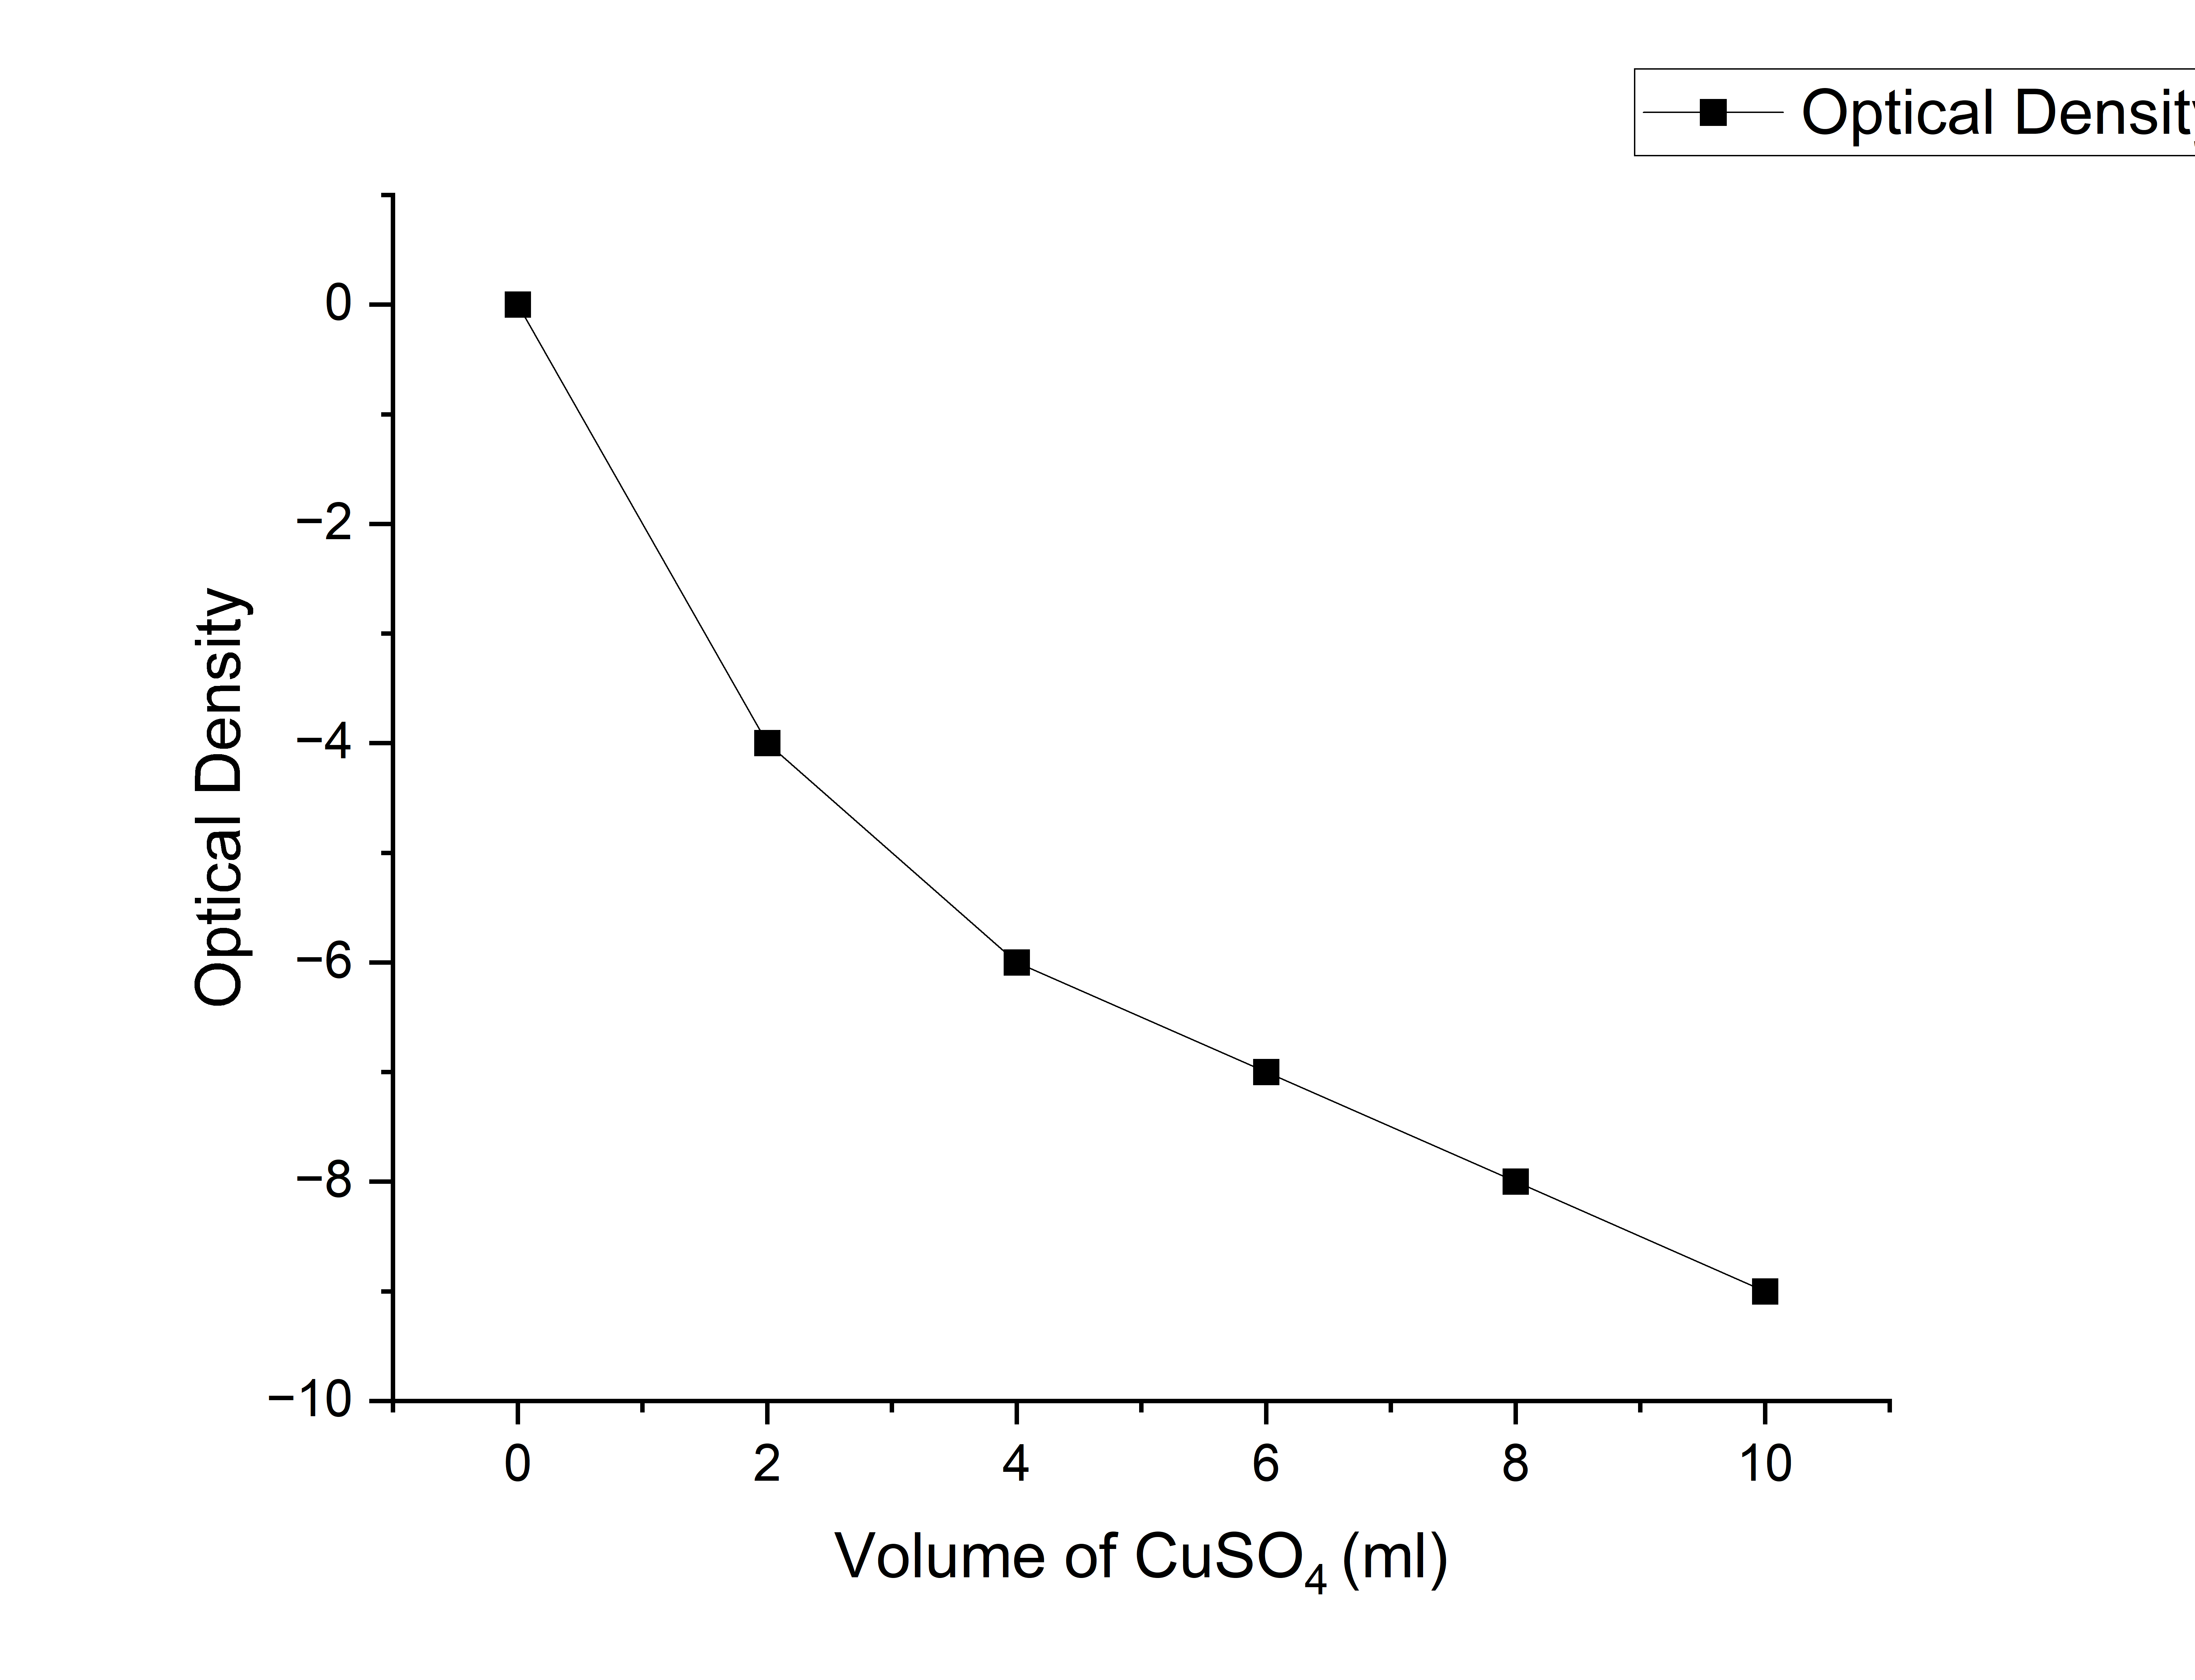
\includegraphics[width = 15cm]{calorimetry.png}
    \caption{Variation of optical density with volume of $CuSO_4$ added}
\end{figure}

\section*{Result}
The absorption vs volume of $CuSO_4$ solution is plotted

\chapter*{Conductometric titration}
\addcontentsline{toc}{chapter}{Conductometric titration \toclineinsert{}{30-01-2024}}
\begin{center}
    \LARGE
     \textbf{Date -30-1-2024}
\end{center}

\section*{Aim}
Determine the strength of the given acid

\section*{Principle}

The conductance of a solution of an electrolyte is due to presence of ions. The change in conductance of a solution by addiction or removal of ions may be employed to follow the course of a titration. When a solution of HCl is titrated with NaOH, the reaction may be represented as follows: $H^++Cl^- +Na^+ + OH^- \longrightarrow Na^+ +Cl^-+H_2O$
The conductance of HCl due to presence of $Cl^-$ions and fast moving $H^+$ ions are removed as unionized $H_2O$ molecules. The decrease in conductance will take place until the equivalence is reached. Further addition of alkali sharply increases conductance of solution owning to introduction of free fast moving $OH^-$ ions. Then measured value of conductance of various stages of neutralization is plotted against the volume of alkali added. The point of neutralization and give volume of alkali required to neutralize the acid.
\section*{Procedure}
The given solution is made up to 100ml. Take out 20ml HCl  in a 100ml beaker. The conductivity cell and a glass rod are introduced into it. If the cell is not fully immersed, sufficient water is added. The cell is connected and conductivity of solution is noted. The NaOH is added from burette in small quantities and conductance and volume of NaOH is measured. Find the equivalence point and calculate strength of HCl. The point of intersection of 2 straight line gives equivalent point.

\section*{Observation}
    \begin{table}[H]
\begin{tabular}{|l|l|l|}
\hline
No. & \begin{tabular}[c]{@{}l@{}}Volume of NaOH\\        (ml)\end{tabular} & \begin{tabular}[c]{@{}l@{}}Conductance\\       (ms)\end{tabular} \\ \hline
1   & 0                                                                    & 150                                                              \\ \hline
2   & 1                                                                    & 137                                                              \\ \hline
3   & 2                                                                    & 124                                                              \\ \hline
4   & 3                                                                    & 110                                                              \\ \hline
5   & 4                                                                    & 98                                                               \\ \hline
6   & 5                                                                    & 88                                                               \\ \hline
7   & 6                                                                    & 79                                                               \\ \hline
8   & 7                                                                    & 71                                                               \\ \hline
9   & 8                                                                    & 63                                                               \\ \hline
10  & 9                                                                    & 57                                                               \\ \hline
11  & 10                                                                   & 51                                                               \\ \hline
12  & 11                                                                   & 47                                                               \\ \hline
13  & 12                                                                   & 43                                                               \\ \hline
14  & 13                                                                   & 40                                                               \\ \hline
15  & 14                                                                   & 38                                                               \\ \hline
16  & 15                                                                   & 36                                                               \\ \hline
17  & 16                                                                   & 34                                                               \\ \hline
18  & 17                                                                   & 32                                                               \\ \hline
19  & 18                                                                   & 32                                                               \\ \hline
20  & 19                                                                   & 36                                                               \\ \hline
21  & 20                                                                   & 39                                                               \\ \hline
22  & 21                                                                   & 42                                                               \\ \hline
23  & 22                                                                   & 45                                                               \\ \hline
24  & 23                                                                   & 47                                                               \\ \hline
25  & 24                                                                   & 50                                                               \\ \hline
26  & 25                                                                   & 52                                                               \\ \hline
27  & 26                                                                   & 55                                                               \\ \hline
28  & 27                                                                   & 57                                                               \\ \hline
29  & 28                                                                   & 61                                                               \\ \hline
\end{tabular}
\end{table}

\begin{figure}[H]
    \centering
    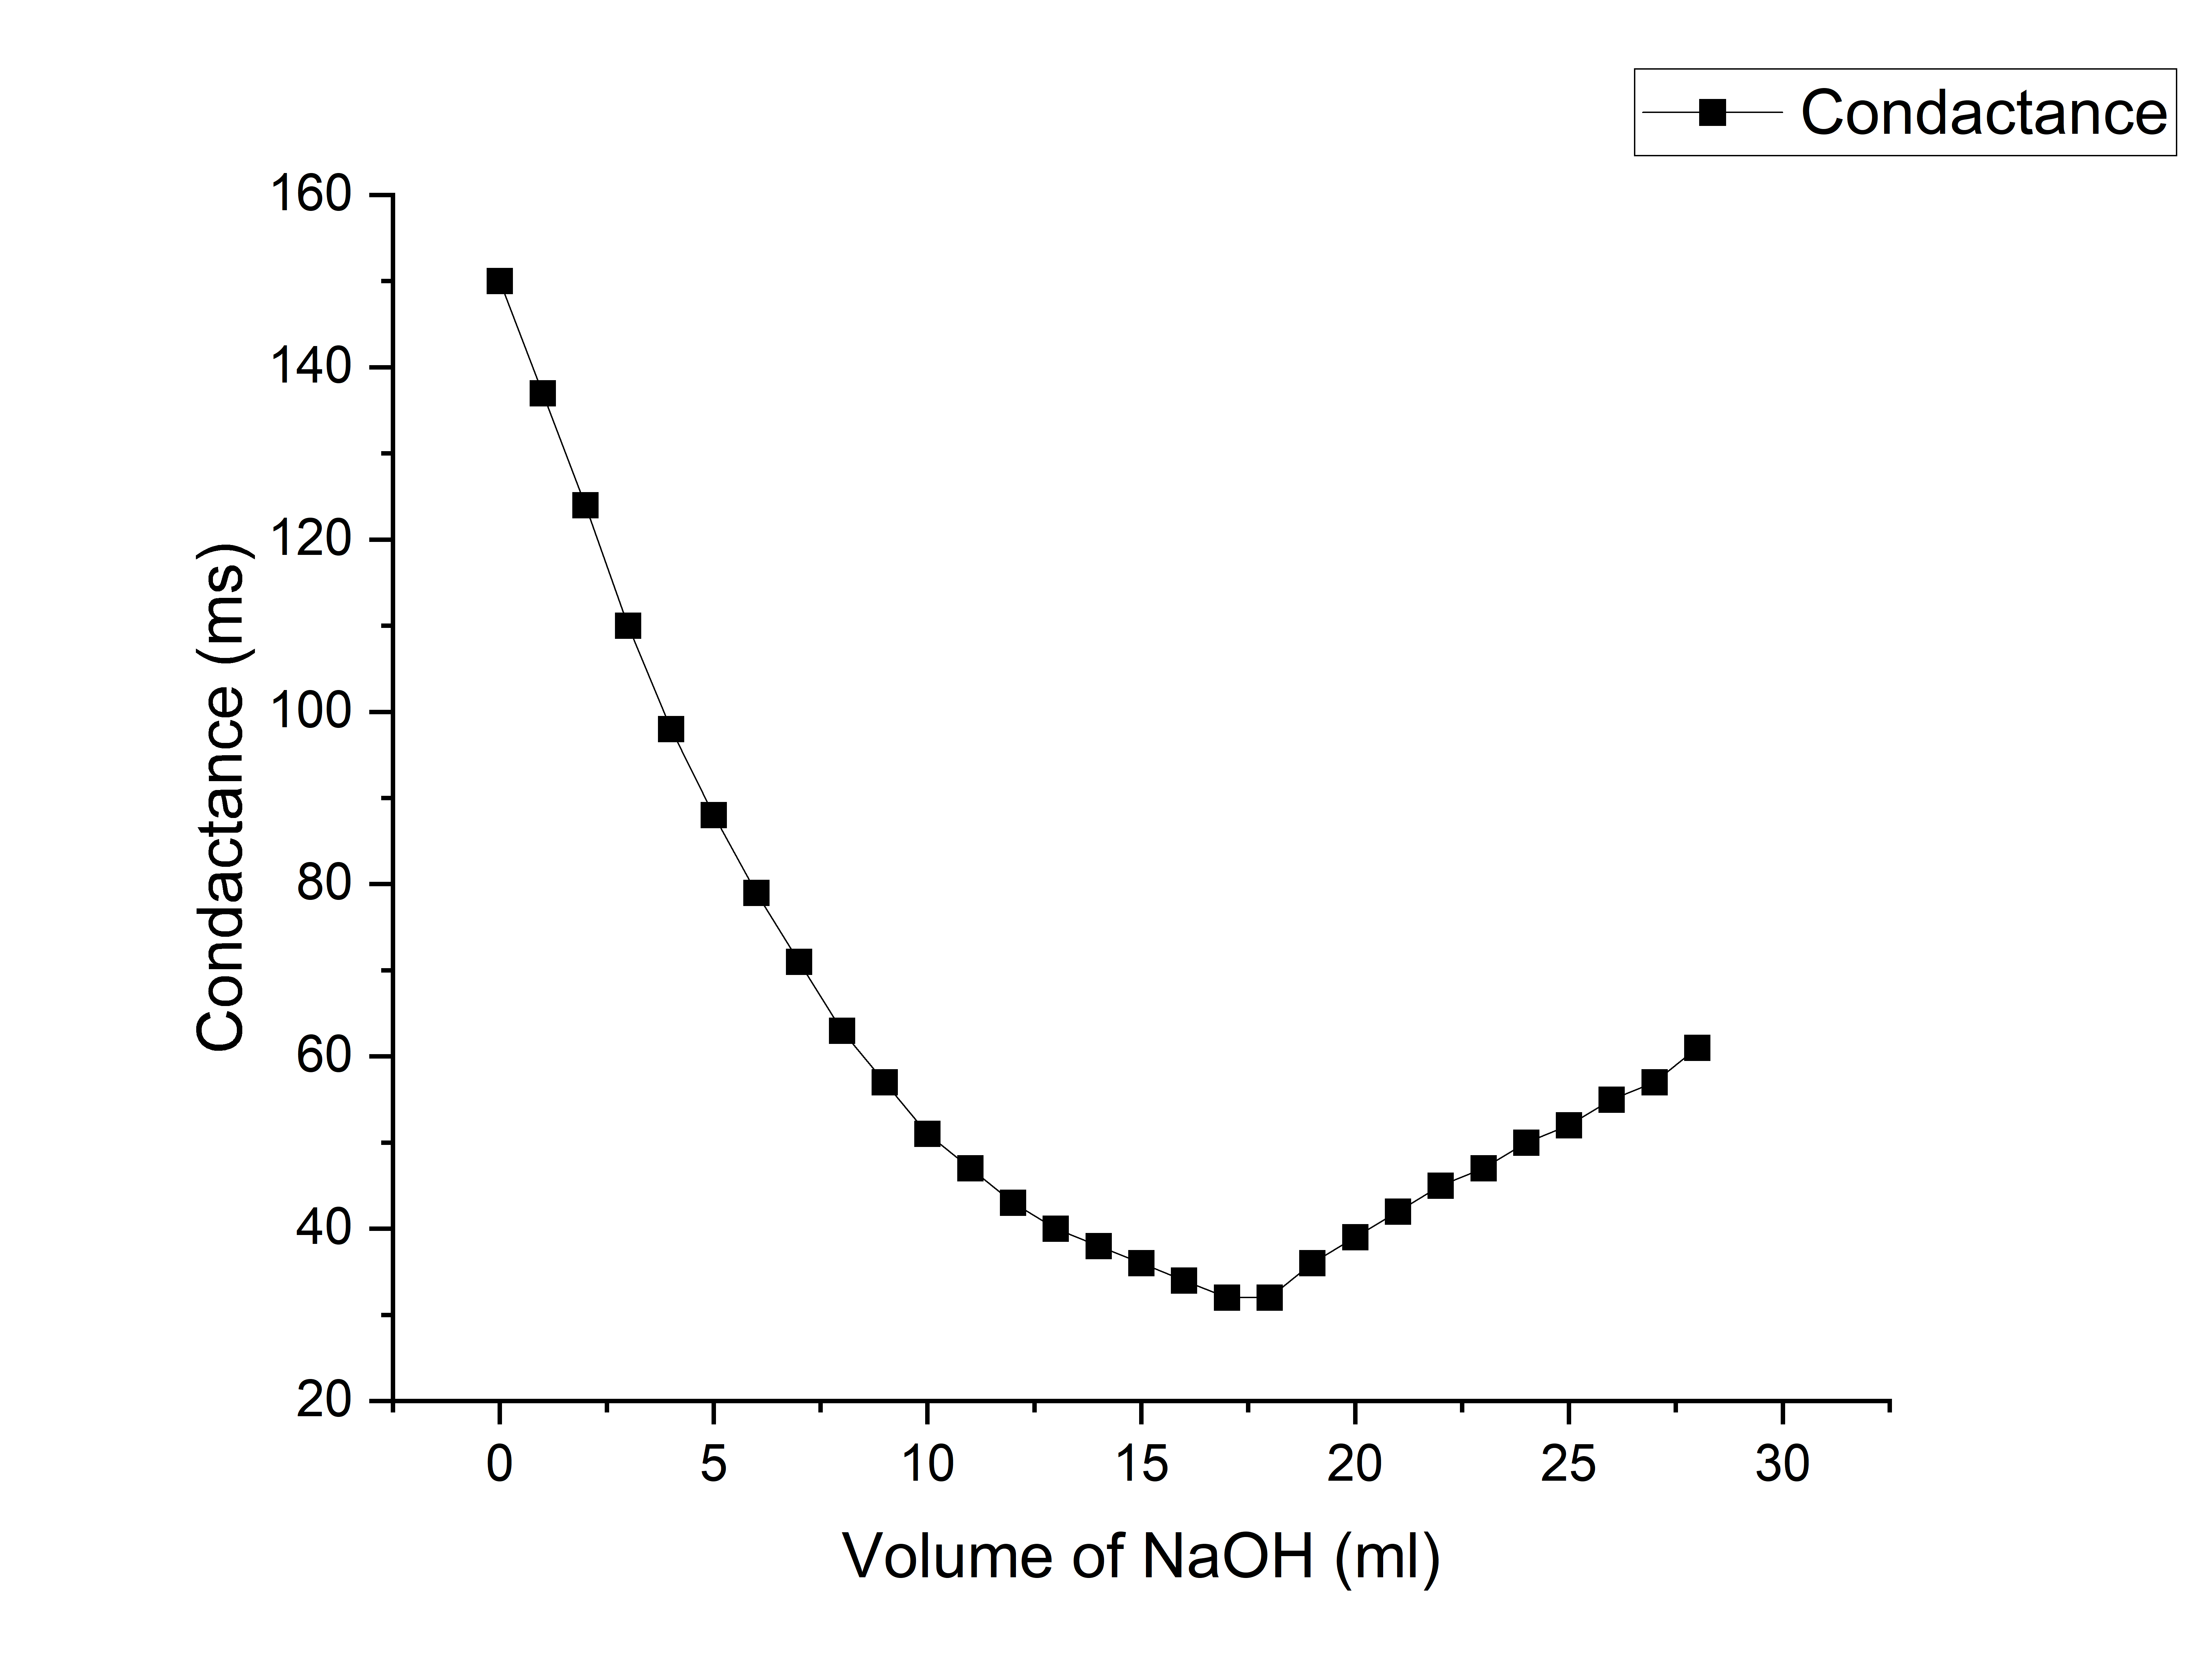
\includegraphics[width = 15 cm]{condactance.png}
    \caption{Variation of condactance with volume of NaOH added}
\end{figure}

\begin{tabular}{l}
    Normality of NaOH = 1.58 N\\
    Normality of NaOH X Volume of NaOH = Normality of HCl X Volume of HCl\\
    0.4 X 18 = N X 20\\
    Normality of HCl = 0.36
\end{tabular}

\section*{Result}
Strength of HCl in given solution = 0.36 N

\chapter*{Determination Of Molecular Mass Of A Compound By Rast's Method}
\addcontentsline{toc}{chapter} {Determination Of Molecular Mass Of A Compound By Rast's Method \toclineinsert{}{15-02-2024}}
\begin{center}
    \LARGE
     \textbf{Date -15-02-2024}
\end{center}

\section*{Aim}
To determine molecular mass of a compound by Rast's method.
\section*{Principle}
When a non volatile solute is dissolved, freezing point of the solvent is lowered. The difference of the freezing point of the pure solvent and the solution is referred as the depression in freezing point and it is related to the molecular mass of the non volatile solute as:\\
\begin{center}
    $\Delta 1000k_f \times w/ M \times W$
\end{center}
where, $\Delta$ is the depression in freezing point\\
$k_f$ is the molar depression constant of solvent\\
$W$ is the mass of the solvent\\
$w$ is the mass of the solute\\
$M$ is the molar mass of solute
\section*{Procedure}
The given solvent(10g) is taken in a boiling tube provided with a stirrer and thermometer. It is corked well and placed in a large beaker of water, which is heated by small flame. The temperature is incresed by about 5$^\circ$C. The tube is then taken out placed in an air jacket. A stop watch is started  and the time-temperature readings recorded every 30 seconds, till the substance freezes. A constant temperature is noted from the graph plotted with time against the temperature.\\
A known weight of solute (0.3 g) is added and transition temperature is determined as above by plotting time-temperature graph. Again about 0.2g of solute is added and experiment is repeated and the freezing point determined from it's cooling curves. Knowing the depression in freezing point, molar mass solute can be determined by using formula
\pagebreak
\section*{Observation}
    \subsection*{Time-Temperature data of Naphthalene}
    \scalebox{1}{
\begin{tabular}{|l|l|}
\hline
\textbf{Time} & \textbf{Temperature} \\ \hline
0             & 82                   \\ \hline
30            & 81.2                 \\ \hline
60            & 80.4                 \\ \hline
90            & 80.2                 \\ \hline
120           & 80                   \\ \hline
150           & 79.8                 \\ \hline
180           & 79.5                 \\ \hline
210           & 79.4                 \\ \hline
240           & 79                   \\ \hline
270           & 78.9                 \\ \hline
300           & 78.8                 \\ \hline
330           & 78.8                 \\ \hline
360           & 78.8                 \\ \hline
390           & 78.7                 \\ \hline
420           & 78.7                 \\ \hline
450           & 78.7                 \\ \hline
480           & 78.8                 \\ \hline
510           & 78.4                 \\ \hline
540           & 78.2                 \\ \hline
570           & 78                   \\ \hline
600           & 78                   \\ \hline
630           & 77.8                 \\ \hline
660           & 77.7                 \\ \hline
690           & 77.5                 \\ \hline
720           & 77.4                 \\ \hline
750           & 77.2                 \\ \hline
780           & 77                   \\ \hline
810           & 76.6                 \\ \hline
840           & 76.5                 \\ \hline
870           & 76.2                 \\ \hline
900           & 76                   \\ \hline
930           & 75.6                 \\ \hline
960           & 75.3                 \\ \hline
990           & 75                   \\ \hline
1020          & 74.8                 \\ \hline
1050          & 74.4                 \\ \hline
\end{tabular}
}
\pagebreak
\subsection*{Time-Temperature data of Naphthalene With 0.3g of acetanilide}
\scalebox{1}{
\begin{tabular}{|l|l|}
\hline
\textbf{Time} & \textbf{Temperature} \\ \hline
\textbf{0}    & 91                   \\ \hline
30            & 87.5                 \\ \hline
60            & 84.6                 \\ \hline
90            & 82.2                 \\ \hline
120           & 80.5                 \\ \hline
150           & 79.1                 \\ \hline
180           & 78.6                 \\ \hline
210           & 78.6                 \\ \hline
240           & 78.6                 \\ \hline
270           & 78.6                 \\ \hline
300           & 78.5                 \\ \hline
330           & 78.4                 \\ \hline
360           & 78.3                 \\ \hline
390           & 78.1                 \\ \hline
420           & 78                   \\ \hline
450           & 78                   \\ \hline
480           & 78                   \\ \hline
510           & 78                   \\ \hline
540           & 77.9                 \\ \hline
570           & 77.8                 \\ \hline
600           & 77.7                 \\ \hline
630           & 77.5                 \\ \hline
660           & 77.4                 \\ \hline
690           & 77.4                 \\ \hline
720           & 77.4                 \\ \hline
750           & 77.4                 \\ \hline
780           & 77.3                 \\ \hline
810           & 77.2                 \\ \hline
840           & 77                   \\ \hline
870           & 77                   \\ \hline
900           & 76.8                 \\ \hline
930           & 76.5                 \\ \hline
960           & 76.4                 \\ \hline
990           & 76.4                 \\ \hline
1020          & 76.3                 \\ \hline
1050          & 76                   \\ \hline
1080          & 75.8                 \\ \hline
1110          & 75.5                 \\ \hline
1140          & 75.3                 \\ \hline
1170          & 75                   \\ \hline
\end{tabular}
}
\\
\pagebreak
\subsection*{Time-Temperature data of Naphthalene With 0.5g of acetanilide}
\scalebox{1}{
\begin{tabular}{|l|l|}
\hline
\textbf{Time} & \textbf{Temperature} \\ \hline
\textbf{0}    & 91.1                 \\ \hline
30            & 87                   \\ \hline
60            & 84                   \\ \hline
90            & 82                   \\ \hline
120           & 80                   \\ \hline
150           & 78.7                 \\ \hline
180           & 78.2                 \\ \hline
210           & 78.2                 \\ \hline
240           & 78.2                 \\ \hline
270           & 78.2                 \\ \hline
300           & 78.2                 \\ \hline
330           & 78.1                 \\ \hline
360           & 78                   \\ \hline
390           & 77.9                 \\ \hline
420           & 77.8                 \\ \hline
450           & 77.7                 \\ \hline
480           & 77.7                 \\ \hline
510           & 77.6                 \\ \hline
540           & 77.5                 \\ \hline
570           & 77.9                 \\ \hline
600           & 77.4                 \\ \hline
630           & 77.3                 \\ \hline
660           & 77.1                 \\ \hline
690           & 77                   \\ \hline
720           & 76.9                 \\ \hline
750           & 76.9                 \\ \hline
780           & 76.8                 \\ \hline
810           & 76.5                 \\ \hline
840           & 76.5                 \\ \hline
870           & 76.3                 \\ \hline
900           & 76                   \\ \hline
930           & 75.9                 \\ \hline
960           & 75.8                 \\ \hline
990           & 75.7                 \\ \hline
1020          & 75.5                 \\ \hline
1050          & 75.4                 \\ \hline
1080          & 75.3                 \\ \hline
1110          & 75.3                 \\ \hline
1140          & 75                   \\ \hline
1170          & 75                   \\ \hline
\end{tabular}
}
\begin{center}
    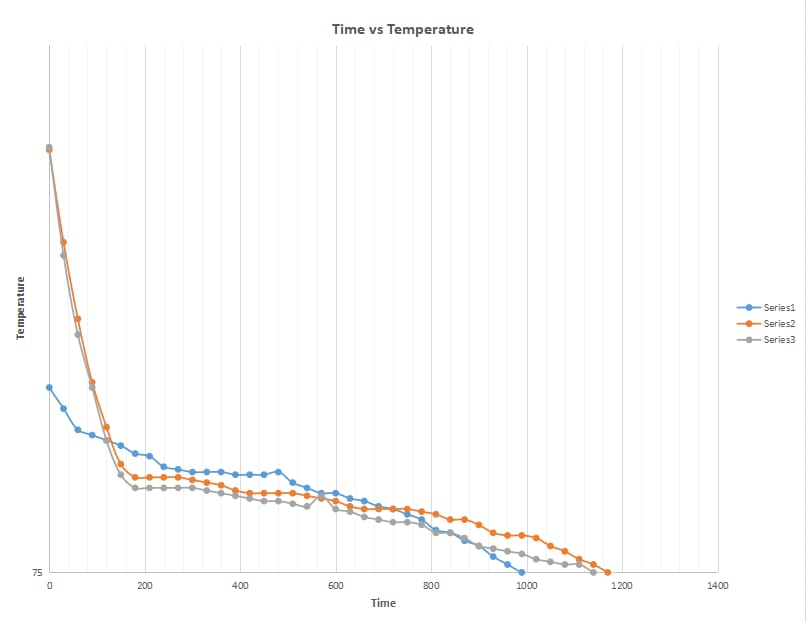
\includegraphics[scale= 0.5]{rast.jpg}
\end{center}
Melting point of Naphthalene - $80 \degree C$
Melting point of 0.2g of mixture - $78.5 \degree C$
Melting point of 0.5g of mixture - $77.4 \degree C$

\section*{Result}
Strength of HCl in given solution = 0.36 N

\end{document}